% 18 variables in here:
% h_1 = 10.0, h_2 = 10.0, h_3 = 10.0, h_4 = 10.0, h_5 = 10.0, h_6 = 10.0, ux_1 = 0.0, ux_2 = 0.0, ux_3 = 0.0, ux_4 = 0.0, ux_5 = 0.0, ux_6 = 0.0, uy_1 = 0.0, uy_2 = 0.0, uy_3 = 0.0, uy_4 = 0.0, uy_5 = 0.0, uy_6 = 0.0
\begin{figure}[h!]
\centering
  \subfigure[Heights are  $h_2=h_3=h_4=h_5=h_6=10$, $h_1$ ranges from 8 to 12.] {
    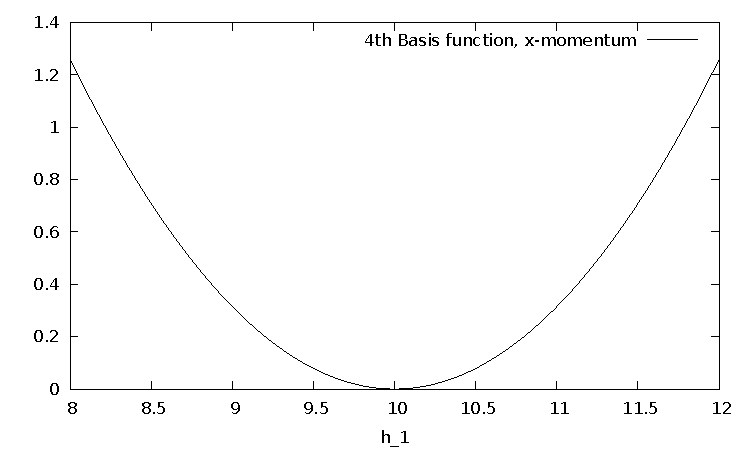
\includegraphics[scale=\zoomfactor]{{{ord2_magnitude_10_default/y_10.0_10.0_10.0_10.0_10.0_0.0_0.0_0.0_0.0_0.0_0.0_0.0_0.0_0.0_0.0_0.0_0.0f06}}}
  }
  % \subfigure[] {
  %   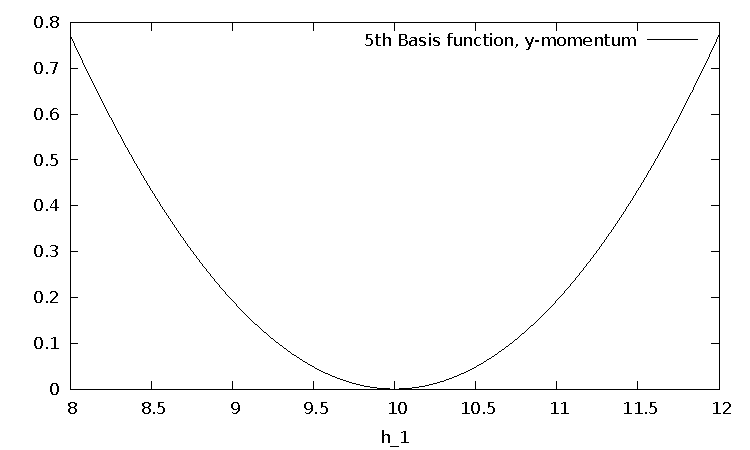
\includegraphics[scale=\zoomfactor]{{{ord2_magnitude_10_default/y_10.0_10.0_10.0_10.0_10.0_0.0_0.0_0.0_0.0_0.0_0.0_0.0_0.0_0.0_0.0_0.0_0.0f09}}}
  % }
  \subfigure[Heights are  $h_2=h_3=h_4=h_5=h_6=1000$, $h_1$ ranges from 998 to 1002.] {
    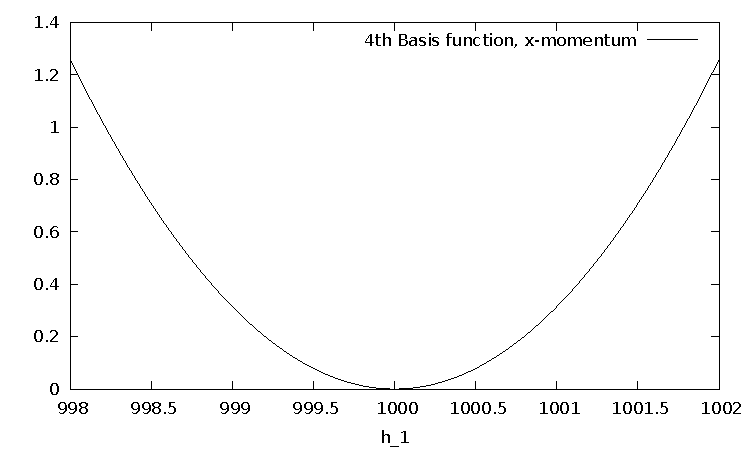
\includegraphics[scale=\zoomfactor]{{{ord2_magnitude_1000_default/y_1000.0_1000.0_1000.0_1000.0_1000.0_0.0_0.0_0.0_0.0_0.0_0.0_0.0_0.0_0.0_0.0_0.0_0.0f06}}}
  }
  % \subfigure[] {
  %   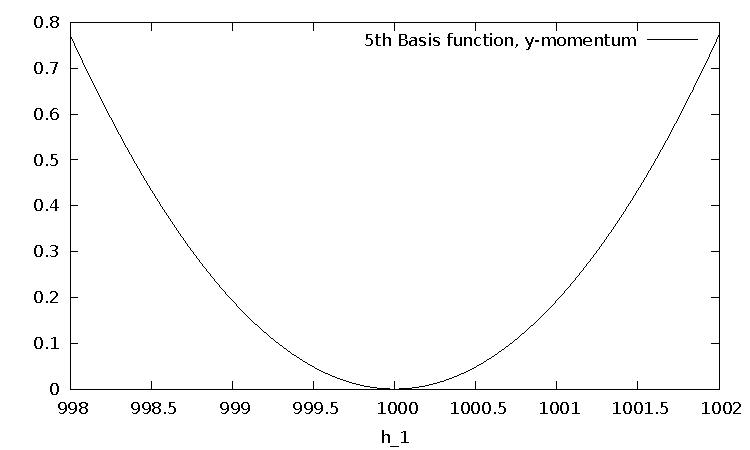
\includegraphics[scale=\zoomfactor]{{{ord2_magnitude_1000_default/y_1000.0_1000.0_1000.0_1000.0_1000.0_0.0_0.0_0.0_0.0_0.0_0.0_0.0_0.0_0.0_0.0_0.0_0.0f09}}}
  % }
\caption{Comparison of different orders of magnitude for the heights for second order basis functions. All momentums are set to 0.}
\label{fig:ord2_magnitude_comparison_default}
\end{figure}

%%% Local Variables:
%%% TeX-master: "../results.tex"
%%% End:
